\documentclass[a4paper,11pt]{article}

\usepackage{amsmath, amssymb, amstext, amsfonts, mathrsfs}


% \sffamily %schrift ohne Serifen

\usepackage[T1]{fontenc} 
% schriftencodierung f�r umlaute, trennung
% f\"ur Uni
\usepackage[latin1]{inputenc}
\usepackage{selinput}
% \usepackage[utf8x]{inputenc} 
\usepackage{bibgerm} 
% german bibliography
\usepackage[german]{babel}
%wichtig f�r deutschen Content
\usepackage{ucs}
%erweiterte UTF-8 Unterst�tzung
\usepackage{wrapfig} 
% Paket zur Positionierung einbinden
\usepackage{multirow}
% zusammenfassen von Tabellenzellen
% \usepackage{subscript}
% zum tiefstellen
\usepackage{lscape}
\usepackage{pdflscape}
% zum drehen der Seite
% \usepackage[super]{natbib}
\usepackage[square,sort,comma,numbers]{natbib}
% Erstellung es Literaturverzeichnisses
\usepackage{url}
% Umbruch f�r URL
\usepackage{pst-3dplot}
% f�r tex Grafiken n�tig
\usepackage{pstricks}
\usepackage{listings}
% f�r das einf�gen von Quelltext
\definecolor{codegray}{rgb}{0.92,0.92,0.92}
\lstset{basicstyle=\fontsize{9}{11}\selectfont\ttfamily, breaklines=true, backgroundcolor=\color{codegray}, numbers=left, numberstyle=\tiny, tabsize=4, language=java}
\definecolor{mymauve}{rgb}{0.58,0,0.82}
\definecolor{mygreen}{rgb}{0,0.6,0}
\lstset{
commentstyle=\color{mygreen},
keywordstyle=\color{mymauve},
language=Java,
stringstyle=\color{blue}
}


%Einstellungen f�r Quellcode
\usepackage[a4paper, left=3cm, right=2cm, top=2cm]{geometry}
% Formatierung R�nder
\usepackage[section]{placeins}
% f�r Floatbarriere
\usepackage{color}
\usepackage{colortbl}
%f�r die Verwendung von Farben

\clubpenalty = 10000 
\widowpenalty = 10000
\displaywidowpenalty = 10000
%Verhinderung von Hurenkindern und Schusterjungen
%10000 bedeutet die sie sollen kommplett vermieden werden

\title{Entwicklung einer Android-Applikation f�r die Alarmierung der Einsatzkr�fte der Freiwilligen Feuerwehren}

\author{Sebastian Rieger}

\pagenumbering{arabic}
%Seitenzahlen(arabische Zahlen)

\setlength{\parindent}{0.25cm} 
%Absatzeinzug �ndern in Zoll
\setlength{\parskip}{0.25cm}
%Absatzabstand
\linespread {1.5}
%Zeilenabstand

\usepackage{setspace}
\usepackage{hyperref}
%anklickbare Hyperlinks

%funktioniert nicht bei Fu�noten
\usepackage{graphicx}
\usepackage{graphics}
%f�r einbinden von Grafiken

\usepackage{framed}
%f�r Umrandung der Erkl�rung
\usepackage{acronym}
% f�r abk�rzungen
% \usepackage{PSTricks}
\usepackage{epstopdf}
% f�r eps bilder nutze pdflatex --shell-escape this.tex
\usepackage{amssymb}
% f�r mathematische Symbole

\usepackage{hyperref}
% klickbare links

% \usepackage{pdfpages}
\usepackage{rotating}
\usepackage{svg}
%%%%%%%%%%%%%%%%%%%%%%%%%%%%%%%%%%%%%%%%%%%%%%%%%%%%%%%%%%%%%%%%%%%%%%%%%%%%%%%%%%%%%%%%%%%%%%%%%%%%%
%% Angaben zur Arbeit
%%%%%%%%%%%%%%%%%%%%%%%%%%%%%%%%%%%%%%%%%%%%%%%%%%%%%%%%%%%%%%%%%%%%%%%%%%%%%%%

\newcommand{\Autor}{Sebastian Rieger}
\newcommand{\MatrikelNummer}{10286908}
\newcommand{\Kursbezeichnung}{TINF12B1}

\newcommand{\FirmenName}{PDV Systeme}
\newcommand{\FirmenStadt}{Erfurt}
\newcommand{\FirmenLogoDeckblatt}{{\includegraphics[width=3cm]{}}}

% Falls es kein Firmenlogo gibt:
%  \newcommand{\FirmenLogoDeckblatt}{}

\newcommand{\BetreuerFirma}{Prof. Rolf Kruse}
\newcommand{\BetreuerDHBW}{Prof. Steffen Avemarg}
\newcommand{\Titel}{Entwicklung eines Natural User Interface mit Hilfe moderner AR und AI Technologien}
\newcommand{\AbgabeDatum}{15.11.2017}

\newcommand{\Dauer}{24 Wochen}

% \newcommand{\Abschluss}{Bachelor of Engineering}
\newcommand{\Abschluss}{Master of Science}

\newcommand{\Studiengang}{Angewandte Informatik}
% \newcommand{\Studiengang}{Angewandte Informatik}
\newcommand{\Was}{Masterarbeit}

%%%%%%%%%%%%%%%%%%%%%%%%%%%%%%%%%%%%%%%%%%%%%%%%%%%%%%%%%%%%%%%%%%%%%%%%%%%%%%%%%%%%%%%%%%%%%%%%%%%%% 
%steuervariable
\usepackage{ifthen} %Package f�r if/else
\newboolean{bilder} %Deklaration
\setboolean{bilder}{true} %Zuweisung
% \setboolean{bilder}{false} %Zuweisung
%%%%%%%%%%%%%%%%%%%%%%%%%%%%%%%%%%%%%%%%%%%%%%%%%%%%%%%%%%%%%%%%%%%%%%%%%%%%%%%%%%%%%%%%%%%%%%%%%%%%%

\lstdefinelanguage{JavaScript}{
  keywords={typeof, new, true, false, catch, function, return, null, catch, switch, var, if, in, while, do, else, case, break},
  keywordstyle=\color{blue}\bfseries,
  ndkeywords={class, export, boolean, throw, implements, import, this},
  ndkeywordstyle=\color{darkgray}\bfseries,
  identifierstyle=\color{black},
  sensitive=false,
  comment=[l]{//},
  morecomment=[s]{/*}{*/},
  commentstyle=\color{purple}\ttfamily,
  stringstyle=\color{red}\ttfamily,
  morestring=[b]',
  morestring=[b]"
}


\makeatletter
\newcommand\footnoteref[1]{\protected@xdef\@thefnmark{\ref{#1}}\@footnotemark}
\makeatother

\begin{document}

\begin{center}
\vspace*{-2cm}
\hfill\includegraphics[width=4cm]{Bilder/logo_FHE}\\[1cm]
{\Huge \Titel}\\[2cm]
{\Huge\scshape \Was}\\[2cm]
% {\large f�r die Pr�fung zum}\\[0.5cm]
% {\Large \Abschluss}\\[0.5cm]
% {\large des Studienganges \Studiengang}\\[0.5cm]
{\large \Studiengang}\\[0.5cm]
{\large an der}\\[0.5cm]
{\large Fachhochschule Erfurt}\\[0.5cm]
{\large von}\\[0.5cm]
{\large\bfseries \Autor}\\[1cm]
{\large Abgabedatum \AbgabeDatum}
\vfill
\end{center}
\begin{tabular}{l@{\hspace{1cm}}l}
Bearbeitungszeitraum             & \Dauer                       \\
Matrikelnummer                   & \MatrikelNummer              \\
% Kurs                             & \Kursbezeichnung             \\
% Ausbildungsfirma                 & \FirmenName                  \\
%                                  & \FirmenStadt                 \\
Betreuer der Masterarbeit    & \BetreuerFirma               \\
Zweitbetreuer der Masterarbeit     & \BetreuerDHBW                \\
\end{tabular}

\newpage
%Seitenumbruch
%%%%%%%%%%%%%%%%%%%%%%%%%%%%%%%%%%%%%%%%%%%%%%%%%%%%%%%%%%%%%%%%%%%%%%%%%%%%%%
%% Descr:       Vorlage für Berichte der DHBW-Karlsruhe, Erklärung
%% Author:      Prof. Dr. Jürgen Vollmer, vollmer@dhbw-karlsruhe.de
%% $Id: erklaerung.tex,v 1.2 2010/07/22 13:30:27 vollmer Exp $
%%%%%%%%%%%%%%%%%%%%%%%%%%%%%%%%%%%%%%%%%%%%%%%%%%%%%%%%%%%%%%%%%%%%%%%%%%%%%%%

% In Bachelorarbeiten muss eine schriftliche Erklärung abgegeben werden. In allen anderen
% Arbeiten entf�llt diese. Hierin best�tigen die Studierenden, dass die Bachelorarbeit
% selbst�ndig verfasst und s�mtliche Quellen und Hilfsmittel angegeben sind. Diese Erkl�rung
% bildet das zweite Blatt der Arbeit. Der Text dieser Erkl�rung muss auf einer separaten Seite
% wie unten angegeben lauten.

\newpage
\thispagestyle{empty}
\begin{framed}
\begin{center}
\Large\bfseries Erkl\"arung
\end{center}

\noindent
Ich, \Autor, versichere hiermit, dass ich die vorliegende Masterarbeit mit dem
Thema
"`\Titel"'
selbstst�ndig und nur unter Verwendung der angegebenen Quellen und Hilfsmittel angefertigt
habe.

\vspace{3cm}
\noindent
\underline{\hspace{4cm}}\hfill\underline{\hspace{6cm}}\\
Ort~~~~~Datum\hfill Unterschrift\hspace{4cm}
\end{framed}

%%%%%%%%%%%%%%%%%%%%%%%%%%%%%%%%%%%%%%%%%%%%%%%%%%%%%%%%%%%%%%%%%%%%%%%%%%%%%%%
\endinput
%%%%%%%%%%%%%%%%%%%%%%%%%%%%%%%%%%%%%%%%%%%%%%%%%%%%%%%%%%%%%%%%%%%%%%%%%%%%%%%

\newpage
\begin{spacing}{0.9}

%Einf�gen Inhaltsverzeichnis
\tableofcontents
\newpage
\section{Abstract}
\newpage
\section{Einleitung}
In den letzten zwanzig Jahren hat sich die Bedienung von Computern grundlegend ge�ndert. Vor nicht all zu vielen Jahren gab es nur die M�glichkeit mit Hilfe von Maus und Tastatur mit einem Computer zu interagieren. 

Mit dem Aufkommen von Touch-Screens jedoch �nderte sich auch die Benutzung von Computern. Es war nun m�glich, direkt mit dem Bildschirm zu interagieren ohne den Umweg �ber die Maus.

Als dann wenig sp�ter die ersten Sprachsteuerungen auf den Markt kamen, �nderte sich die Interaktion mit dem Computer erneut. So ist es nun m�glich, Computern mittels Sprache Befehle zu erteilen oder Texte zu sprechen, welche automatisch transkribiert werden.

Heute ist es mit manchen Smartphones schon m�glich, Nachrichten wie SMS zu schreiben und zu versenden, ohne das Telefon �berhaupt in die Hand zu nehmen. Dies ist nur durch neuste Entwicklungen in der \ac{KI} m�glich.

Im selben Zeitraum hat sich parallel auch die \ac{VR} entwickelt. Sie versucht Menschen mit Hilfe von verschiedenen Brillen in eine virtuelle Welt zu versetzen. Die Entwicklungen solcher \ac{VR} Systeme wurde vor allem von der Spieleindustrie getrieben, da sie immer neue Versuche unternimmt, Spieler besser in die Welt des Spiels zu versetzen. 

Eine Abstufung der \ac{VR} ist die \ac{AR}, welche versucht die analoge, reale Welt um digitale Inhalte zu erweitern. Hierbei sind die M�glichkeiten f�r den Einsatz von \ac{AR} fast unbegrenzt. 
Es ist also quasi m�glich, jede menschliche T�tigkeit durch die \ac{AR} zu unterst�tzen. 

Genau hier setzt der Schwerpunkt der Arbeit an. Im Verlauf soll versucht werden, ein \ac{NUI} unter Zuhilfenahme moderner \ac{AR} und \ac{KI} Technologien zu erstellen.

Hierf�r werden aktuelle \ac{AR} und \ac{KI} Systeme daraufhin untersucht, wie sie im Zusammenspiel ein \ac{NUI} bilden k�nnen, welches allein durch Sprache und Gesten mit einem Computer interagiert.

Es soll eine �bliche T�tigkeit mit Hilfe einer \ac{AR} Technologie in der realen Welt abgebildet werden, welche dann von einem Menschen nur unter Zuhilfenahme von Sprache und Gesten gesteuert und bearbeitet werden kann.
\newpage
\section{Natural User Interfaces}
Als Natural User Interfaces \ac{NUI} werden Benutzeroberfl�chen von Computern und Programmen bezeichnet, welche sich durch Gesten, Sprache, Ber�hren, Tippen und Wischen bedienen lassen. In der heutigen Zeit begegnen wir st�ndig solchen \ac{NUI}s, zum Beispiel beim mehrmals t�glichen Griff zum Smartphone oder der Smartwatch. �ber einen ber�hrungsempfindlichen Display, werden Apps heute schon �ber Gesten gesteuert. \cite{InteraktiveSysteme}

Diese Steuerung funktioniert zum Teil bei der j�ngeren Generation, so genannten "`digital natives"', also Menschen welche im digitalen Zeitalter geboren sind, schon automatisch und unterbewusst. Jeder, der schon einmal eine App bediente kennt die Geste zum l�schen aus einer Liste! Die Bewegung des Eintrags nach links oder rechts l�scht das entsprechende Element getreu nach dem Motto "`Aus den Augen aus dem Sinn"'. \cite{WikiDigitalNativ}

Diese Art von Gesten ist so intuitiv f�r Menschen, dass auch "`digital immigrants"', also Menschen, die erst im Erwachsenenalter den Umgang mit digitalen Ger�ten gelernt haben, diese nach einmaliger Erkl�rung gelernt.

Aber das nat�rliche Verhalten von uns Menschen geht noch viel weiter. Diese einmal auf einem Smartphone gelernte Geste in einer App wird unterbewusst auch auf andere Applikationen �bertragen. Eine App, welche diese einfache und mittlerweile etablierte Geste nicht unterst�tzt, wird umgehend Kritik ernten, da sie mit altbekanntem bricht und so ein "`Nat�rliches"' arbeiten nicht mehr gegeben ist.

\subsection{Nat�rliche Bedienung durch Gesten}
Was jedoch genau macht eine Geste "`Nat�rlich"'? Die Beantwortung dieser Frage ist im gleichen Ma�e trivial wie komplex. 

Dies bedeutet, sobald einmal eine "`Nat�rliche Geste"' gefunden wurde, erscheint wie gegeben und wird nicht in Frage gestellt, weil sie ja "`Logisch"' ist. Das Komplexe ist jedoch, solche "`logischen Gesten"', erst einmal zu finden. 

Hierf�r m�ssen viele Aspekte aus den Verhaltenswissenschaften beachtet werden:
\begin{itemize}
\item Arbeitswissenschaft
\item Psychologie
\item Soziologie
\item P�dagogik
\end{itemize}

Erg�nzend zu diesen Aspekten gibt es die EN ISO 9241, welche Richtlinien der Mensch-Computer-Interaktion beschreibt. Insbesondere der Teil 110 "`Grunds�tze der Dialoggestaltung"' kann helfen passende Bedienm�glichkeiten f�r ein \ac{NUI} zu finden. \cite{ISO9241} Die Grunds�tze sind:

\begin{itemize}
\item Aufgabenangemessenheit - geeignete Funktionalit�t, Minimierung unn�tiger Interaktionen 
\item Selbstbeschreibungsf�higkeit - Verst�ndlichkeit durch Hilfen / R�ckmeldungen 
\item Steuerbarkeit - Steuerung des Dialogs durch den Benutzer 
\item Erwartungskonformit�t - Konsistenz, Anpassung an das Benutzermodell 
\item Fehlertoleranz - unerkannte Fehler verhindern nicht das Benutzerziel, erkannte Fehler sind leicht zu korrigieren 
\item Individualisierbarkeit - Anpassbarkeit an Benutzer und Arbeitskontext 
\item Lernf�rderlichkeit - Minimierung der Erlernzeit, Metaphern, Anleitung des Benutzers 
\end{itemize}

\subsection{Erstellung eines Use Cases}
Anhand dieser Grunds�tze kann nicht nur ein System, welches mit Tastatur und Maus bedient wird, definiert werden sondern auch ein \ac{NUI}. Dies wird nun beispielhaft an der Geste f�r "`l�schen"' gezeigt, um sicher zu Stellen, dass im sp�teren Verlauf der Arbeit ein \ac{NUI} anhand genau dieser Grunds�tze definiert werden kann.

\paragraph{Aufgabenangemessenheit} 
Das Wischen zum L�schen eines Eintrags ist schnell und einfach zu erlernen. Ebenso kann die Geste schnell wiederholt werden, um m�glichst schnell auch mehrere Elemente l�schen zu k�nnen.

\paragraph{Selbstbeschreibungsf�higkeit}
Die Geste ist zwar einfach und mittlerweile auch bekannt, aber es muss auch sichergestellt sein, dass neue Nutzer die Geste lernen k�nnen. Dies kann zum Beispiel durch ein kurzes wackeln beim ersten �ffnen angezeigt werden. Dem Nutzer wird durch diese Bewegung suggeriert, dass diese Elemente bewegbar sind. 

\paragraph{Steuerbarkeit}
Wischt der Nutzer nun bewusst oder durch Neugier ausgel�st vom Wackeln das Element aus dem Bildschirm, muss immer die M�glichkeit bestehen, das Element wiederherstellen zu k�nnen. Dies ist nur konsequent, da eine so einfache Geste auch einmal versehentlich gemacht werden kann.

\paragraph{Erwartungskonformit�t}
Ist diese Geste einmal etabliert, muss sie konsequent in allen Listen implementiert sein, da es sonst zum Bruch der Erwartung kommt und der Nutzer unn�tiger verwirrt wird.

\paragraph{Fehlertoleranz} 
Zu Fehlertoleranz geh�rt das wiederherstellen eines Eintrags wie schon unter Steuerbarkeit beschrieben. Zus�tzlich kommt jedoch hinzu, dass die Geste eventuell vom Ger�t falsch interpretiert wurde und der Nutzer gar nichts l�schen wollte. Auch in solchen F�llen muss eine Wiederherstellung m�glich sein.

\paragraph{Individualisierbarkeit}
Das Wischen ist eine tolle Geste! Aber in welche Richtung muss gewischt werden? Nach links oder rechts wischen zum l�schen? Genau hier muss die App schlau reagieren, denn die richtige Antwort ist: Beides muss m�glich sein. Bekannterma�en gibt es Links- und Rechtsh�nder, wobei das Ger�t zumeist mit der dominanten Hand gehalten wird. F�r einen Rechtsh�nder, welcher den Daumen zum wischen links hat, ist das Wischen nach rechts leichter als nach links. Genau umgekehrt ist es bei Linksh�ndern. Diese wischen eher nach Links. 

Dieses Verhalten kann auch selbst nachgestellt werden, egal ob der Nutzer Links- oder Rechtsh�nder ist. Die Geste wird unterbewusst durch beide H�nde in unterschiedliche Richtungen ausgef�hrt. 

\paragraph{Lernf�rderlichkeit}
Bei der  Lernf�rderlichkeit trifft ganz klar das Sprichwort "'Aus den Augen aus dem Sinn"` zu. Der Nutzer m�chte etwas "'weg"` haben. Warum es also nicht au�erhalb des Displays platzieren? Es wird nicht mehr gesehen und ist somit "'weg"`. Diese einfache Analogie ist f�r jeden Nutzer zu verstehen und umzusetzen.

\subsection{Auswertung des Use Cases}
Anhand des vorgestellten Use Cases wurde gezeigt, dass es m�glich ist ein \ac{NUI} zu designen. Hierbei m�ssen nat�rlich die Gegebenheiten des jeweiligen Ger�tes beachtet werden, wie zum Beispiel, dass ein Smartphone in beiden H�nden gehalten werden kann. Dadurch kann sich gegebenen Falls der Use Case erweitern oder ver�ndern. 

1991 beschrieb Mark Weiser schon, wie sich Computer immer mehr in unseren Alltag integrieren und langsam immer unkenntlicher werden. Die Grenze zwischen realer Umwelt und virtueller Welt verschwimmt heute immer mehr. \cite{Computer21}

Dies hat nat�rlich auch zur Folge, das sich die Schnittstelle zwischen Mensch und Computer st�ndig �ndert und weiterentwickelt. Musste man 1997 zu beginn von Google noch Stichworte mit Maus und Tastatur eingeben um das Internet zu durchsuchen, reicht heute schon ein Sprachbefehl. 

Der Computer wertet mit verschiedenen Algorithmen das gesprochene aus und versucht dem Nutzer eine direkte Antwort zu geben, w�hrend man 1997 von Google eine Liste mit Webseiten bekam, auf welchen die Schlagworte zu finden waren. 
\newpage
\section{Augmented Reality}
In der heutigen Zeit ist fast jedem der Begriff Augmented Reality gel�ufig. Jedoch gibt es im wissenschaftlichen Umfeld keine einheitliche Definition. Georg Klein definiert die \ac{AR} als "`Anreicherung der realen Welt um computergenerierte Zusatzobjekte"'. \cite{KleinG}

Viele Abhandlungen zu diesem Thema beziehen sich auf das "`Reality-Virtuality Continuum"', welches von Milgram, Takemura, Utsumi und Kishino welches in Abbildung \ref{rvc_img} zu sehen ist. Dieses stellt bildlich dar, wie sich eine \ac{AR}-Anwendung einordnen l�sst. Links ist die reale Umgebung (Real Environment) und rechts die Virtuelle Umgebung (Virtual Environment) zu sehen. 

Heutige \ac{VR}-Anwendungen m�ssen also ganz rechts eingeordnet werden. Zwischen der realen und der virtuellen Umgebung gibt es jedoch noch weitere Abstufungen. So gibt es die "`Augmented  Reality"', welche die reale Welt um virtuelle Elemente erg�nzt. Sie bezieht sich eher auch die reale Umgebung, weshalb sie weitere links angeordnet ist. Die "`Augmented Virtuality"' ist das genaue Gegenteil der \ac{AR}. Hier wird die virtuelle Welt des Computers um reale Gegenst�nde erg�nzt. 

Im wissenschaftlichen Umfeld wird als Oberbegriff f�r "`Augmented Reality"' und "`Augmented Virtuality"' oft "`Mixed Reality"' oder "`Enhanced Reality"' verwendet. \cite{ARTuP}

\begin{figure}[!ht]
\centering
\includegraphics[width=10cm]{Bilder/ar_vr.png}
\caption{Reality-Virtuality Continuum \cite{rvc}}
\label{rvc_img}
\centering
\end{figure}

Der Begriff der \ac{AV} ist heute weniger gebr�uchlich, da es keine wirklichen Anwendungsfelder gibt, in denen eine virtuelle Welt um reale Gegenst�nde erg�nzt werden muss. Im Umkehrschluss wird heute jedoch die \ac{AR} immer bedeutender, da bei fast jeder menschlichen T�tigkeit eine Unterst�tzung durch Computergenerierte Objekte oder Informationen m�glich ist. 

Im medizinischen Umfeld, k�nnen �rzten zum Beispiel Positionen von empfindlichen Gewebe oder zu entfernenden Fremdk�rpern bei einer Operation angezeigt werden. Eine andere Einsatzm�glichkeit w�re das unterst�tzende Anzeigen von Gefahren oder Fluchtwegen f�r Feuerwehrleute, die sich einem stark verrauchten Brandobjekt befinden. Computer k�nnen durch Infrarot und W�rmebild das Sichtverm�gen eines Feuerwehrmannes in einer Gefahrensituation so entscheidend erh�hen um sich selbst und andere zu retten.

\subsection{Typen von visuelle Ausgabeger�te}
Im folgenden Abschnitt werden m�gliche visuelle Ausgabeger�tetypen genauer beschrieben und auf ihre Einsatzm�glichkeiten untersucht. 

\subsubsection{Handheld-Ger�te}
Als Handheld werden in Ger�te bezeichnet, die wie der Name schon sagt von einer Person in der Hand gehalten werden. Im \ac{AR}-Umfeld sind hier Smartphones oder Tablets gemeint, welche heutzutage durch ihre Dual- oder Quad-Core-Prozessoren und teilweise mehrere Gigabyte RAM in der Lage sind, auch komplexere \ac{AR}-Anwendungen zur Ausf�hrung zu bringen. 

In Smartphones und Tablets nimmt die Kamera das Bild der realen Welt auf und stellt es in Echtzeit auf dem Display dar. Ein Programm (App) ist dann in der Lage, die aufgenommene reale Welt um virtuelle Elemente zu erweitern und diese innerhalb des Kamerabildes auf dem Bildschirm zu platzieren. 

Hierbei ergibt sich jedoch ein Problem, da sich der Blickwinkel es Betrachters vom Blickwinkel der Kamera unterscheidet, was zu einer unsauberen Platzierung der Objekte im Bild f�hrt.
In Abbildung \ref{hh_blick_img} ist zu sehen, wie sich der Blickwinkel der Kamera und der Blickwinkel des Betrachters unterscheiden.

\begin{figure}[!ht]
\centering
\includegraphics[width=10cm]{Bilder/hh_blick.png}
\caption{Unterschiedliche Blickfelder von Betrachter und Kamera bei Handheld-AR \cite{VuAR}}
\label{hh_blick_img}
\centering
\end{figure}

Um den unterschied, zwischen den Blickwinkeln auszugleichen, muss das entsprechende Ger�t die beiden Blickwinkel aufeinander abstimmen. Dies kann jedoch kein zur Zeit auf dem Markt befindliches Ger�t leisten. 

Einen ersten Ansatz herzu hat die University of California gemacht, indem sie ein Tablet mit einem Kinect Sensor verbunden haben. Mit Hilfe des zus�tzlichen Sensors und dem "`KinectFusion Algorithmus"' konnten sie eine "`Magic Lens"' entwickeln, die beide Blickwinkel in etwa aufeinander abstimmt. \cite{MagicLens}

In Abbildung \ref{magic_lens_img} ist einmal der Unterschied zwischen einer Aufnahme mit Magic Lens und ohne schematisch dargestellt. 

Im linken Bildabschnitt ist gut zu sehen, das B�ume und andere Gegenst�nde im Bildschirm exakt an der Position in der realen Welt liegen. Im Gegensatz dazu sind B�ume und andere Gegenst�nde im rechten Bildabschnitt merklich verzerrt. 

\begin{figure}[!ht]
\centering
\includegraphics[width=10cm]{Bilder/magic_lens.png}
\caption{Schematische Darstellung des Magic Lens Effekts \cite{VuAR}}
\label{magic_lens_img}
\centering
\end{figure}

Ein weiteres Problem ist, das \ac{AR}-Anwendungen f�r die optimale Skalierung und Platzierung von virtuellen Objekten im Raum zus�tzlich Tiefeninformationen des aktuellen Bildes ben�tigen, denn nur dann ist auch gew�hrleistet, dass virtuelle Objekte in der richten Gr��e im realen Raum positioniert werde. 

Dieses Problem versucht gerade das Projekt Tango von Google zu l�sen. Mit Hilfe eines Lasers und einer Infrarotkamera k�nnen Tiefeninformationen zum aktuellen Bild aufgenommen und verarbeitet werde. \cite{Tango} 

Nur mit der Tango Technologie ist es bisher m�glich, AR-Objekte richtig skaliert und im richtigen Blickwinkel pr�zise im Raum zu positionieren.  Weitergehende Informationen sind auf den Developer-Seiten\footnote{\url{https://get.google.com/tango/}} von Google zu finden. Bisher unterst�tzen jedoch nur das "`Lenovo Phab2"' und das "`Asus ZenFon AR"' diese Technologie, da hier eine zus�tzliche Sensoreinheit im Smartphone verbaut sein muss.

Abschlie�en kann �ber \ac{AR}-Anwendungen ausgesagt werden, das sie Grunds�tzlich lauff�hig auf Handheld Ger�ten wie Tablets oder Smartphones sind. Die Bedingungen sind jedoch nicht zumindest heutzutage noch optimal, wie eben dargelegt wurde.

\subsubsection{Video-See-Through-Displays}
Video-See-Through Ger�te existieren im Vergleich zu \ac{AR}-Anwendungen schon ziemlich lange. Schon Anfang der 1940er Jahre wurde erste Head-Up-Displays in Kampfflugzeugen eingesetzt, um die Piloten mit zus�tzlichen Informationen zu versorgen, welche immer im Blick behalten werden m�ssen. \cite{WikiHeadup} 

Von Anfang an, wurden die zus�tzlichen Informationen auf eine Glasfl�che Projiziert, um das Sichtfeld nicht unn�tig einzuschr�nken. Es wurde entweder direkt auf das Cockpit Fenster Projiziert oder die Piloten hatten kleine durchsichtige Displays in den Helm eingearbeitet, auf die mit Hilfe von Spiegeln Projiziert werden konnte.

Mit der Ver�ffentlichung des iPhones im Jahre 2007 wurde das Thema \ac{AR} immer interessanter, da mit ihm die technische Grundlage gelegt wurde. 2008 erschien der \ac{AR}-Browser Wikitude wodurch das Feld immer mehr Fu� fasste und sich nun rasant weiter entwickelt.
\cite{entwicklerAR}

Die durch die immer gr��erer Verbreitung von \ac{AR}-Anwendungen wurde auch die Hardware entsprechend weiterentwickelt und angepasst, was zu den ersten \ac{AR}-Brillen f�hrte.

Durch die Kombination von Handheld-Ger�ten und Head-Up-Displays entstanden bis 2014 die ersten Video-See-Through-Brillen oder auch \ac{AR}-Brillen genannt. Die Entwicklung dieser Brillen steckt noch in den Kinderschuhen, aber dennoch gibt es schon zwei auf dem Markt verf�gbare Ger�te, die f�r die sp�tere Entwicklung eines \ac{NUI} in Betracht gezogen werden k�nnen. Zum einen ist das die Epson Moverio BT-200 und zum anderen die Microsoft HoloLens, welche zur Zeit nur f�r Entwickler verf�gbar ist.

Die HoloLens und die Moverio sind beide Prismen basiert. In Abbildung \ref{prisma_img} ist die Funktionsweise von Prismen basierten See-Through-Displays schematisch Dargestellt. Ein normales Display ist an einer Seite eines Prismas angebracht. Das Prisma leitet das Licht des Displays weiter, so das es in das Auge des Betrachters weitergeleitet wird. Weil das Prisma nach vorn durchsichtig ist, wird auch das Umgebungslicht direkt in das Auge des Betrachters geleitet. Innerhalb des Prismas vermischen sich die beiden Bilder, wobei das Displaylicht das Umgebungslicht �berlagert. F�r den Betrachter sieht es somit aus, als w�rden die Objekte in der realen Welt zu finden sein.

\begin{figure}[!ht]
\centering
\includegraphics[width=14cm]{Bilder/prisma.png}
\caption{Schematische Darstellung des Aufbaus eines See-Through-Displays \cite{VuAR}}
\label{prisma_img}
\centering
\end{figure}

\paragraph{Die Microsoft HoloLens}
wurde 2015 von Microsoft vorgestellt und ist momentan die Wahrscheinlich beste \ac{AR}-Brille auf dem Markt. Sie verf�gt �ber mehrere Kameras und Tiefensensoren, womit die HoloLens in der Lage ist sich selbstst�ndig im Raum zu orientieren. 

\begin{wrapfigure}{r}{4cm}
\centering
\includegraphics[width=4cm]{Bilder/hololens.jpg}
\caption{Aufgesetzte HoloLens \cite{WikiHolo}}
\label{holo_img}
\vspace{-10pt}
\end{wrapfigure}

Ausgestattet mit einem Intel Atom x5-Z810 Prozessor und 2 Gigabyte RAM, ist die Brille sehr gut aufgestellt und kann Programme und Berechnungen ohne zus�tzliche Hardware ausf�hren. Als Betriebssystem kommt Windows 10 zum Einsatz. Die Akkulaufzeit wird mit zwei Stunden angegeben, wobei dies wie immer Abh�ngig von der geforderten Leistung ist. \cite{ARVRHolo}

F�r Entwickler hat Microsoft ein \ac{SDK} bereitgestellt mit dessen Hilfe es m�glich ist Anwendungen f�r die HoloLens zu entwickeln. \cite{MSHolo}

�ber verschiedene Sensoren kann die HoloLens Bewegungen und Gesten des Nutzers wahrnehmen, erkennen und verarbeiten.

Die HoloLens ist standardm��ig in der Lage, grundlegende Gesten zu erkennen, mit denen zum Beispiel ein Tippen, Halten, Rotieren und Zoomen m�glich ist.
Auf genauere technische Details zur Programmierung der HoloLens wird im Kapitel ????? genauer eingegangen.

Eine Besonderheit der HoloLens ist nat�rlich das mit Microsoft ein gro�er Softwarekonzern hinter der Entwicklung steht und somit ein schnelles voranschreiten der Technik quasi sicher ist.

\paragraph{Die Epson Moverio BT-200}

\subsection{Auswertung der M�glichkeiten f�r ein Natural User Interface}
\newpage
\section{Artificial Intelligence}
Als \ac{AI} oder im deutschen auch \emph{artifizielle Intelligenz} oder \emph{k�nstliche Intelligenz}, bezeichnet, in der Informatik, ein System welches eine Automatisierte Intelligenz besitzt. Eine eindeutige Definition f�r \ac{AI} gibt es nicht, da es schon in der Psychologie an einer genauen Definition mangelt. \cite{WikiKI}

In der heutigen Zeit werden Systeme und Algorithmen die auf neuronalen Netzen basieren als ann�hernd intelligent bezeichnet. Ein Beispiel hierf�r ist "`Google Translate"' welches zwischen verschiedenen Sprachen mittels neuronalen Netz �bersetzt. \cite{TranslateKI}

Es gibt aber auch intelligente Systeme wie "`IBM Watson"', welche nicht auf neuronalen Netzen basieren und ann�hernd intelligent wirken. Diese Intelligenz ist das Resultat einer sehr gro�en Wissensbasis und verschiedenen kombinatorischen Algorithmen. Um zu zeigen wie Leistungsf�hig Watson ist, trat er 2011 in der Quizshow "`Jeopardy"' an und gewann gegen die weltbesten Spieler. \cite{IBMWatson}

Im allgemeinen Sprachgebrauch werden als \ac{AI} heute �blichen Sprachassistenten wie Siri, Alexa, Cortana oder Google Assistent bezeichnet. Das im Verlauf der Arbeit zu entwickelnde \ac{NUI} soll auf einen dieser Assistenten aufbauen.

Die Entwicklung einer eigenen Spracherkennung ist im Rahmen dieser Arbeit nicht m�glich, da dies sehr viel Zeit und Arbeit in Anspruch nimmt. Selbst Firmen wie Google oder Amazon ben�tigten mehrere Jahre um ihre Assistent auf das aktuelle Leistungsniveau zu heben.

Es soll nun untersucht werden, in wie weit die heute g�ngigen Assistenten genutzt werden k�nnen, um eine Sprachsteuerung f�r ein \ac{NUI} (siehe Kapitel ?????) umzusetzen.

Hierbei muss der Assistent folgende Kriterien erf�llen:
\begin{itemize}
 \item Lauff�gig auf der Microsoft HoloLens
 \item Offene Programmierschnittstelle (\ac{SDK})
 \item M�glichkeit eigener Sprachkomandos
\end{itemize}

\subsection{Funktionsweise der Sprachassistenten}
Auch wenn die genauen Implementierungen der Sprachassistenten verschiedenen ist, so haben sie alle eins gemenisam und zwar ist dies der Weg der Sprachverarbeitung.

Die Funktionsweise von Siri udn Co. ist recht einfach gehalten. Der Nutzer l�st mit einem Stichwort "`Hey, Siri..."', "`Ok, Google..."' und so weiter die Benutzung aus. Der darauf folgende Sprachbefehl wird aufgezeichnet und komprimiert an einen Server weitergeleitet, welcher den gesprochenen Text auswertet und in schriftliche Befehle umwandelt. Diese Befehle werden dann umgehend zur�ck an das Endger�t des Nutzers Versand, welches nun auf die Befehle reagieren kann.

\begin{figure}[!ht]
\centering
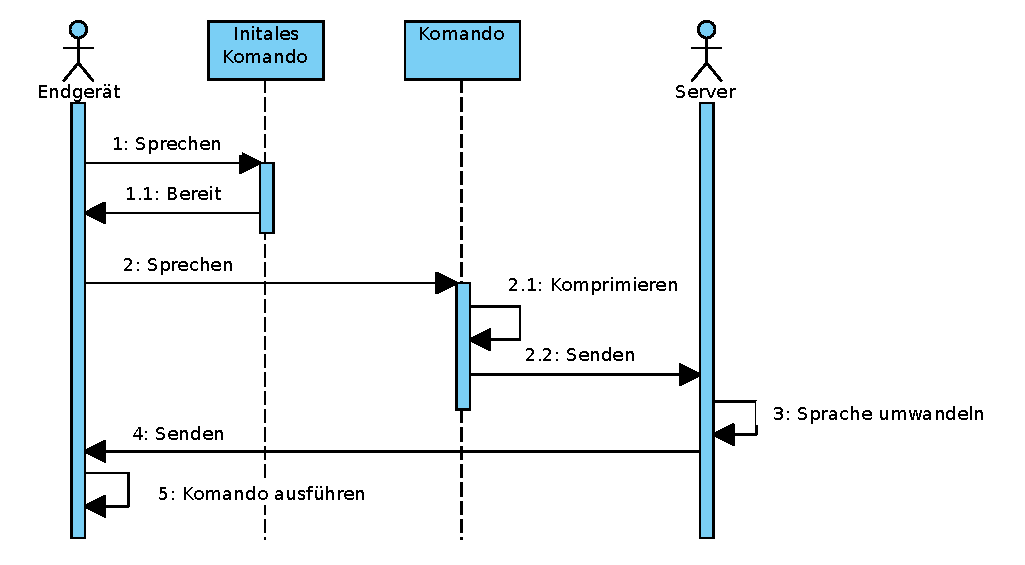
\includegraphics[width=14cm]{Bilder/Assistenten.eps}
\caption{Schematische Darstellung der Kommunikation von Sprachassistenten}
\label{assistent_img}
\centering
\end{figure}

Hierbei ist zu beachten, dass jegliche Kommunikation zwischen Endger�t und Server bei allen Assistenten �ber HTTPS gesichert ist.

Innerhalb der Server, welche die Sprache zu Text wandeln, kommen fast immer neuronale Netze zum einsatz, da nur sie in der Lage sind schnell und eindeutig die Spachbefehle zu wandeln.
Durch die geh�ufte Verwendung mit immer neuen Stimmen und Befehlen lernen die Systeme immer mehr hinzu und k�nnen so die Anfragen immer schneller und besser umwandeln. Dies hat zur Folge, das ein System besser wird, je h�ufiger es genutzt wird.

In den nun folgenden Abschnitten werden die genannten Assistenten auf ihre M�glichkeiten untersucht.

\subsection{Siri}
Der wohl �lteste und bekannteste Sprachassistent ist "`Siri"'. Siri ist eine Software zur Spracherkennung und wurde von Apple im Jahre 2010 zusammen mit der Firma Siri Inc. von Apple aufgekauft. Schon ein Jahr sp�ter wurde der Assistent im Zuge der Ver�ffentlichung des iPhone 4s vorgestellt und ver�ffentlicht.

Siri ist eine propriet�re Software und nur iOS, machOS, watchOS und tvOS einsetzbar, weshalb eine Verwendung auf der HoloLens nicht m�glich ist. Zwar verf�gt Siri �ber ein offenes \ac{SDK}, dieses ist jedoch nur f�r Apple eigene Betriebssysteme ausgelegt.


\subsection{Alexa}
\subsection{Cortana}
\subsection{Google Assistent}

\subsection{Auswertung der M�glichkeiten}

\section{Beschreibung eines Natural User Interface}
\subsection{Use Case}
\subsection{Anforderungsanalyse}
\section{Konzept}
\section{Versuch der Entwicklung eines Natural User Interface anhand der Microsoft HoloLens und ...}
\section{Fazit}
\section{Zusammenfassung}


\end{spacing}

\newpage
\section{Abk�rzungsverzeichnis}
\begin{acronym}
  \acro{KI}{\emph{k�nstliche Intelligenz}}
  \acro{VR}{\emph{Virtuelle Realit�t}}
  \acro{AR}{\emph{Argumented Reality}}
  \acro{NUI}{\emph{Natural User Interface}}
  \acro{AV}{\emph{Augmented Virtuality}}
  \acro{SDK}{\emph{Software Development Kit}}
\end{acronym}
\newpage
\listoffigures
\newpage
\listoftables
% Abk�rzungsverzeichnis
\newpage
\bibliographystyle{alpha}
% verzeichnis im DIN format
\bibliography{Quellen}
\end{document}
